%\documentclass[a4paper, 12pt]{mwrep}
\documentclass[12pt,a4paper]{article}
\usepackage[polish]{babel}
\usepackage[T1]{fontenc}
\usepackage[utf8x]{inputenc}
\usepackage{hyperref}
\usepackage{url}
\usepackage[]{algorithm2e}
\usepackage{listings}
\usepackage{graphicx}
\graphicspath{
    {media/}
}

\usepackage{color}
\usepackage{listings}

\lstloadlanguages{% Check Dokumentation for further languages ...
	C,
	C++,
	csh,
	Java
}

\definecolor{red}{rgb}{0.6,0,0} % for strings
\definecolor{blue}{rgb}{0,0,0.6}
\definecolor{green}{rgb}{0,0.8,0}
\definecolor{cyan}{rgb}{0.0,0.6,0.6}

\lstset{
	language=csh,
	basicstyle=\footnotesize\ttfamily,
	numbers=left,
	numberstyle=\tiny,
	numbersep=5pt,
	tabsize=2,
	extendedchars=true,
	breaklines=true,
	frame=b,
	stringstyle=\color{blue}\ttfamily,
	showspaces=false,
	showtabs=false,
	xleftmargin=17pt,
	framexleftmargin=17pt,
	framexrightmargin=5pt,
	framexbottommargin=4pt,
	commentstyle=\color{green},
	morecomment=[l]{//}, %use comment-line-style!
	morecomment=[s]{/*}{*/}, %for multiline comments
	showstringspaces=false,
	morekeywords={ abstract, event, new, struct,
		as, explicit, null, switch,
		base, extern, object, this,
		bool, false, operator, throw,
		break, finally, out, true,
		byte, fixed, override, try,
		case, float, params, typeof,
		catch, for, private, uint,
		char, foreach, protected, ulong,
		checked, goto, public, unchecked,
		class, if, readonly, unsafe,
		const, implicit, ref, ushort,
		continue, in, return, using,
		decimal, int, sbyte, virtual,
		default, interface, sealed, volatile,
		delegate, internal, short, void,
		do, is, sizeof, while,
		double, lock, stackalloc,
		else, long, static,
		enum, namespace, string},
	keywordstyle=\color{cyan},
	identifierstyle=\color{red},
}
\usepackage{caption}
\DeclareCaptionFont{white}{\color{white}}
\DeclareCaptionFormat{listing}{\colorbox{blue}{\parbox{\textwidth}{\hspace{15pt}#1#2#3}}}
\captionsetup[lstlisting]{format=listing,labelfont=white,textfont=white, singlelinecheck=false, margin=0pt, font={bf,footnotesize}}


\addtolength{\hoffset}{-1.5cm}
\addtolength{\marginparwidth}{-1.5cm}
\addtolength{\textwidth}{3cm}
\addtolength{\voffset}{-1cm}
\addtolength{\textheight}{2.5cm}
\setlength{\topmargin}{0cm}
\setlength{\headheight}{0cm}

\begin{document}
	
	\title{Modelowanie i analiza systemów informatycznych\\
			\bigskip
			\large{dokumentacja projektu:} \\
			\large{System wspomagania decyzji}
		}
	\author{inż. Bartosz Ociepka
		\and inż. Beniamin Stecuła}
	\date{\today}
	
	\maketitle







	\newpage
\section*{Podział pracy}
Podział pracy był płynny, lecz z większym naciskiem na:
\begin{itemize}
	\item inż. Bartosz Ociepka -- backend, praktyka,
	\item inż. Beniamin Stecuła -- frontend, teoria, dokumentacja.
\end{itemize}
	
	
	
\section*{Udokumentowanie pracy}
	Dokumentowanie pracy odbyło się na kilka sposobów:
	\begin{itemize}
		\item utworzenie niniejszej dokumentacji,
		\item zarządzanie podziałem i wykonaniem zadań w serwisie Trello,
		\item przechowywanie kopii poprzednich wersji programu.
	\end{itemize}
	
\section*{Instrukcja obsługi}
% TODO instrukcja


	
\section*{Instrukcja wdrożenia}

	Aby wdrożyć projekt należy wykonać poniższą listę kroków:
	
	\begin{enumerate}
		\item zaimportowanie projektu w Visual Studio 2015,
		\item import danych do bazy danych MySql (dołączono plik dump.sql zawierający potrzebne tabele),
		\item zmiana connectionString w kodzie na odpowiadające używanej bazie,
		danych (dokonanie zmiany klas gdy używana jest inna baza niż MySql),
		\item uruchomienie projektu.
	\end{enumerate}
	
\section*{Część testowa}
% TODO testy


	
\section*{Baza danych}
Diagram UML bazy danych został przedstawiony na rysunku \ref{fig:dbdiagram}.


\begin{figure}[h]
	\centering
	\centerline{
	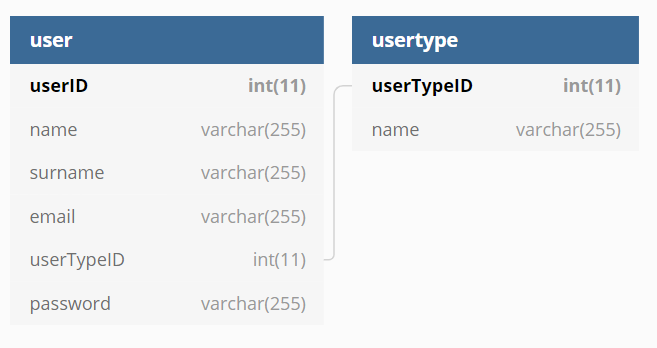
\includegraphics[width=0.9\linewidth]{media/dbdiagram}
	}
	\caption{Diagram klas.}
	\label{fig:dbdiagram}
\end{figure}



\section*{Komponenty systemu}
% TODO komponenty


	
\section*{Algorytm szyfrowania}
	
	
	W naszym programie do rejestracji i logowania użyliśmy stworzonej przez siebie klasy \emph{AuthorizationManager}, która zawiera metody \emph{LogIn(), Register(), LogOut()}.
	Szyfrowanie zaimplementowane zostało w klasie \emph{RSAHelper}, w której znajduje się cała logika szyfrowania opierająca się na klasie \emph{RSACryptoServiceProvider}.
	Do szyfrowania użyty został algorytm RSA. W samej konfiguracji można ustawić haszowanie, szyfrowanie lub zapisywanie haseł w trybie plain text, choć nie jest to zalecane. Po wybraniu rodzaju można wybrać konkretny sposób enkrypcji. Poniżej przykład zmiany haszowania na SHA256 w pliku web.config poprzez atrybut hashAlgorithmType.
	
	\begin{lstlisting}
		
	\end{lstlisting}

	TLS wykorzystuje Algorytm Rivesta-Shamira-Adlemana (RSA) -- jest to jeden z pierwszych i najpopularniejszych asymetrycznych algorytmów kryptograficznych o kluczu publicznym. Może być stosowany i do szyfrowania, i cyfrowego podpisywania plików.
	
	\smallskip
	Polega on na liczeniu funkcji Eulera dla dużych liczb pierwszych, a jego bezpieczeństwo opiera się na trudności faktoryzacji dużych liczb złożonych.
	
	\smallskip
	Każdy z rozmówców posiada parę kluczy: prywatny i publiczny. Pierwszy z nich służy do deszyfrowania wiadomości przychodzącej, a drugi do szyfrowania wychodzącej. Aby nawiązać komunikację rozmówcy muszą wymienić się swoimi kluczami publicznymi. Klucze prywatne nigdy nie są ujawniane.
	
	
\section*{System ekspercki}

	W dziale sztucznej inteligencji systemem eksperckim (Expert System -- ES) nazywa się system komputerowy, który emuluje podejmowanie decyzji przez ludzkiego specjalistę z danej dziedziny. Odzwierciedla procesy myślowe na zasadzie działania ludzkiego mózgu.
	
	Do rozwiązań wykorzystujących ES zaliczamy:
	\begin{itemize}
		\item systemy agentowe,
		\item agenty programowe,
		\item eksplorację danych,
		\item wspomaganie twórczego myślenia,
		\item ontologie systematyzujące wiedzę.
	\end{itemize}
	\bigskip
	
	ES powinien zawierać trzy charakterystyczne, podstawowe cechy:
	\begin{itemize}
		\item bazy wiedzy -- schematycznie zapisane informacje uzyskane od ludzkich ekspertów w danej dziedzinie,
		\item procedury wnioskujące -- odzwierciedlające wnioskowanie symboliczne, które jest charakterystyczne dla funkcjonowania ludzkiego mózgu,
		\item zdolność do poszerzania wiedzy -- umożliwienie ciągłego rozwoju systemu w przypadku stale napływających nowych informacji koniecznych do uwzględnienia aby otrzymywać stale aktualne wyniki zgodne z nowym stanem wiedzy w dziedzinie.
	\end{itemize}
	\bigskip
	
	Struktura ES składa się z sześciu podstawowych elementów:
	\begin{itemize}
		\item baza wiedzy -- składająca się ze zbioru reguł,
		\item baza danych -- zawierająca dane obiektów, wartości, przypadki i hipotezy,
		\item procedury wnioskowania -- jest to maszyna wnioskująca,
		\item procedury objaśniania -- tłumaczą strategię wnioskowania,
		\item procedury sterowania dialogiem -- funkcje wejścia/wyjścia sterujące programem i wyznaczające zadania, które ma wykonać
		\item procedury zarządzania wiedzą -- pozwalają na modyfikację oraz rozszerzanie, pozyskiwanie wiedzy.
	\end{itemize}
	
	
	
	%ES zazwyczaj działa na zasadzie rozpatrywania warunków if-else.
	
	
	
	

\section*{Przykładowy kod z aplikacji z testami}
% TODO kod aplikacji


\begin{lstlisting}
	Tutaj wklejamy pelen kod. 
\end{lstlisting}

\end{document}
